\documentclass{article}
\newcommand{\maru}[1]{\hbox{\raisebox{0.2mm}{\textcircled{\scriptsize \raisebox{-0.1mm}{#1}}}}}

\usepackage{tikz}
\usetikzlibrary{intersections,calc,arrows.meta}
\begin{document}
\noindent
\begin{tikzpicture}
\draw[->,>=stealth,semithick](-2,0)--(2,0)node[above]{$x$};
\draw[->,>=stealth,semithick](0,-2)--(0,2)node[above]{$y$};
\draw(0,0)node[below right]{O};
\draw[very thick,domain=-2:2]plot(\x,0.9);
\end{tikzpicture}
\begin{tikzpicture}
    \draw[->,>=stealth,semithick](-2,0)--(2,0)node[above]{$x$};
    \draw[->,>=stealth,semithick](0,-2)--(0,2)node[above]{$y$};
    \draw(0,0)node[below right]{O};
    \draw[very thick,domain=-2:2](0.9,-2)--(0.9,2);
\end{tikzpicture}\\
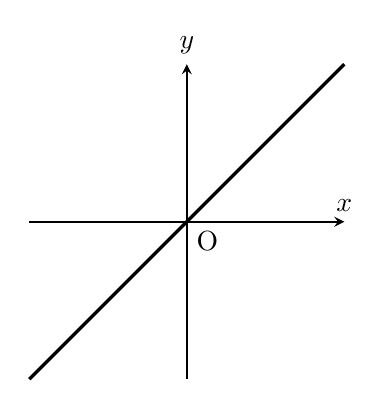
\begin{tikzpicture}
    \draw[->,>=stealth,semithick](-2,0)--(2,0)node[above]{$x$};
    \draw[->,>=stealth,semithick](0,-2)--(0,2)node[above]{$y$};
    \draw(0,0)node[below right]{O};
    \draw[very thick,domain=-2:2]plot(\x,\x);
\end{tikzpicture}
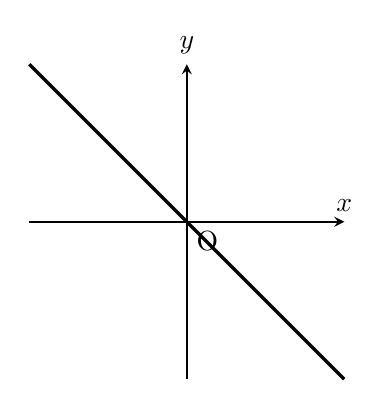
\begin{tikzpicture}
    \draw[->,>=stealth,semithick](-2,0)--(2,0)node[above]{$x$};
    \draw[->,>=stealth,semithick](0,-2)--(0,2)node[above]{$y$};
    \draw(0,0)node[below right]{O};
    \draw[very thick,domain=-2:2]plot(\x,-\x);
    \end{tikzpicture}

\maru{1}
\maru{2}
\maru{3}
\maru{4}
\end{document}